\chapter{Protocolli bus}

\section{Protocolli di comunicazione}
I protocolli di comunicazione standard comprendono protocolli per periferiche e dispositivi di memoria, sono stati principalmente proposti da ARM per applicazione industriali e molti di questi si riferiscono a un dominio di applicazione specifico.

\begin{itemize}
    \item I2C
    \item ARM AXI
    \item ARM AXI Lite
    \item ARM AXI Stream (address less)
\end{itemize}

\subsection{Protocollo I2C ($\text{I}^2\text{C}$)}

Il protocollo I2C, Inter-Integrated Circuit, è stato inizialmente proposto da Philips negli anni 80.

Questo protocollo è altamento diffuso in vari contesti (videocamere, sensori, CPU...) per via della sua semplicità:
\begin{itemize}
    \item protocollo seriale
    \item richiede solo 2 fili
    \item frequenza 100KHz (ora a 400KHz o 1+ MHz)
    \item semplice e lightweight
    \item predecessore di SPI
\end{itemize}

\subsubsection{Funzionamento}
É presente un \textbf{master}, che \textit{inizia sempre la comunicazione}, si hanno un collegamento per i \textbf{dati} (\textbf{SDA}) e uno per il \textbf{clock} (\textbf{SCL}). Si possono avere al massimo 127 slave.

\begin{figure}[H]
    \caption{Schema di collegamento}
    \centering
    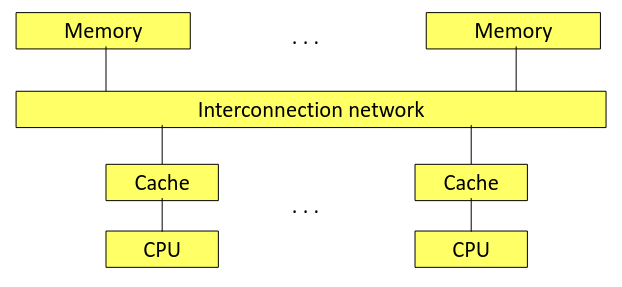
\includegraphics[width=0.6\textwidth]{/home/riccardoob/appunti/sistemi_digitali/images/11.png}
\end{figure}

Ogni ciclo di bus consiste di una sequenza di \textit{due} sezioni:
\begin{itemize}
    \item \textbf{Address Frame}
    \begin{itemize}
        \item \textit{master} trasmette l'\textbf{indirizzo} dello \textit{slave} coinvolto
        \item \textit{master} specifica se è una lettura o una scrittura
    \end{itemize}
    \item \textbf{Data Frame}
    \begin{itemize}
        \item in caso di scrittura, \textit{master} invia i dati allo \textit{slave}
        \item in caso di lettura, \textit{master} legge dati dallo \textit{slave}
    \end{itemize}
\end{itemize}

\begin{figure}[H]
    \caption{Schema di funzionamento}
    \centering
    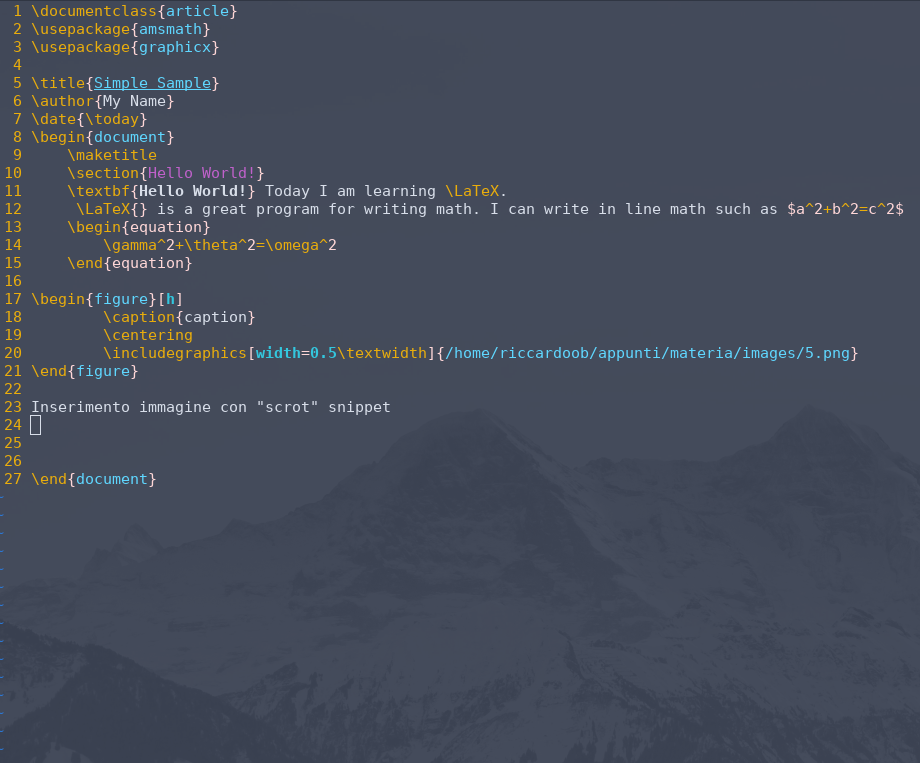
\includegraphics[width=0.8\textwidth]{/home/riccardoob/appunti/sistemi_digitali/images/12.png}
\end{figure}

\subsection{Protocolli on-chip su Zynq}
\begin{itemize}
    \item AXI4: adatto per comunicazioni con dispositivi \textbf{memory-mapped} ad alte prestazioni, può gestire 256 trasferimenti dato un singolo indirizzo (\textit{burst transfer})
    \item AXI4-Lite: abilita un singolo trasferimento per dispositivi \textbf{memory-mapped}.
    \item AXI4-Stream: adatto a per trasferimenti di stream di dati ad alte prestazioni con dispositivi \textbf{non memory-mapped}, spesso utilizzato per gestire stream di immagini o segnali.
\end{itemize}

\subsubsection{Comunicazioni con dispositivi memory-mapped}
\begin{figure}[H]
    \centering
    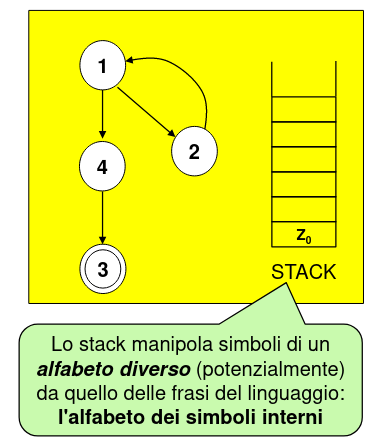
\includegraphics[width=0.5\textwidth]{/home/riccardoob/appunti/sistemi_digitali/images/13.png}
\end{figure}

\subsubsection{Lettura e scrittura \textbf{burst}}
\begin{multicols}{2}
    \begin{multicolfigure}
        \centering
        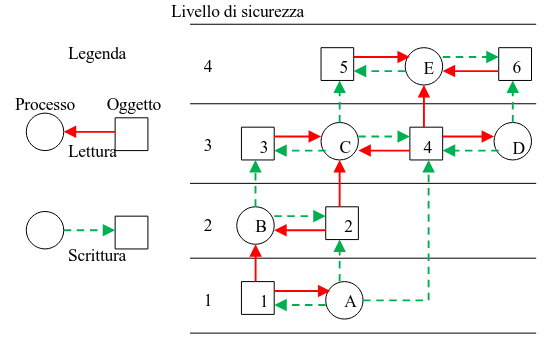
\includegraphics[width=\textwidth]{/home/riccardoob/appunti/sistemi_digitali/images/14.png}
    \end{multicolfigure}
    \columnbreak
    \begin{multicolfigure}
        \centering
        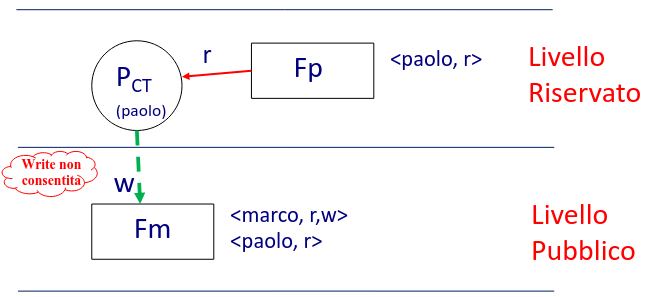
\includegraphics[width=\textwidth]{/home/riccardoob/appunti/sistemi_digitali/images/15.png}
    \end{multicolfigure}
\end{multicols}









